%MÁSTER UNIVERSITARIO EN GESTIÓN SOSTENIBLE DE LA TIERRA Y EL TERRITORIO
%TÉCNICAS DE ANÁLISIS CUANTITATIVAS Y CUALITATIVAS
%DOCUMENTO DE RESOLUCIÓN DEL EJERCICIO 3 DE EVALUACIÓN
%MARCOS RIAL DOCAMPO


\documentclass[11pt,a4paper]{article}

\usepackage[utf8]{inputenc}
\usepackage[spanish]{babel}
\usepackage{amsmath}
\usepackage{amsfonts}
\usepackage{amssymb}
\usepackage{url}
\usepackage[colorlinks,linktocpage=true,citecolor=blue,linkcolor=blue]{hyperref}
\usepackage{booktabs}
\usepackage{graphicx,geometry}
\usepackage{caption}
\usepackage{verbatim,moreverb}

\usepackage{xcolor}
\definecolor{gray97}{gray}{.97}
\definecolor{gray75}{gray}{.75}
\definecolor{gray45}{gray}{.45}
\definecolor{mauve}{rgb}{0.58,0,0.82}
\definecolor{dkgreen}{rgb}{0,0.6,0}

\author{Marcos Rial Docampo}
\title{Técnicas de Análisis Cuantitativas y Cualitativas\\Resolución del ejercicio de evaluación 3}
\date{\small{\today}}

\begin{document}
\maketitle

En este ejercicio de evaluación se nos presentan datos de superficie agrícola abandonada (porcentaje de la superficie agrícola al inicio del periodo), densidad de población ($hab/km^{2}$) y altitud media (metros sobre el nivel del mar) de una serie de 50 observaciones tomadas en otros tantos municipios gallegos.

Lo primero que haremos será suprimir la variable categórica \textit{X} puesto que no ofrece información alguna al tratarse de un código referente a la zona donde se tomaron las observaciones. Una vez hecho esto extraemos graficamente la relación directa entre las tres variables restantes como se muestra en la figura \ref{fig:relacion}. La estimación numérica de la correlación entre estas variables sería la mostrada en el cuadro \ref{tab:matrizcor}.

\begin{figure}
	\centering
	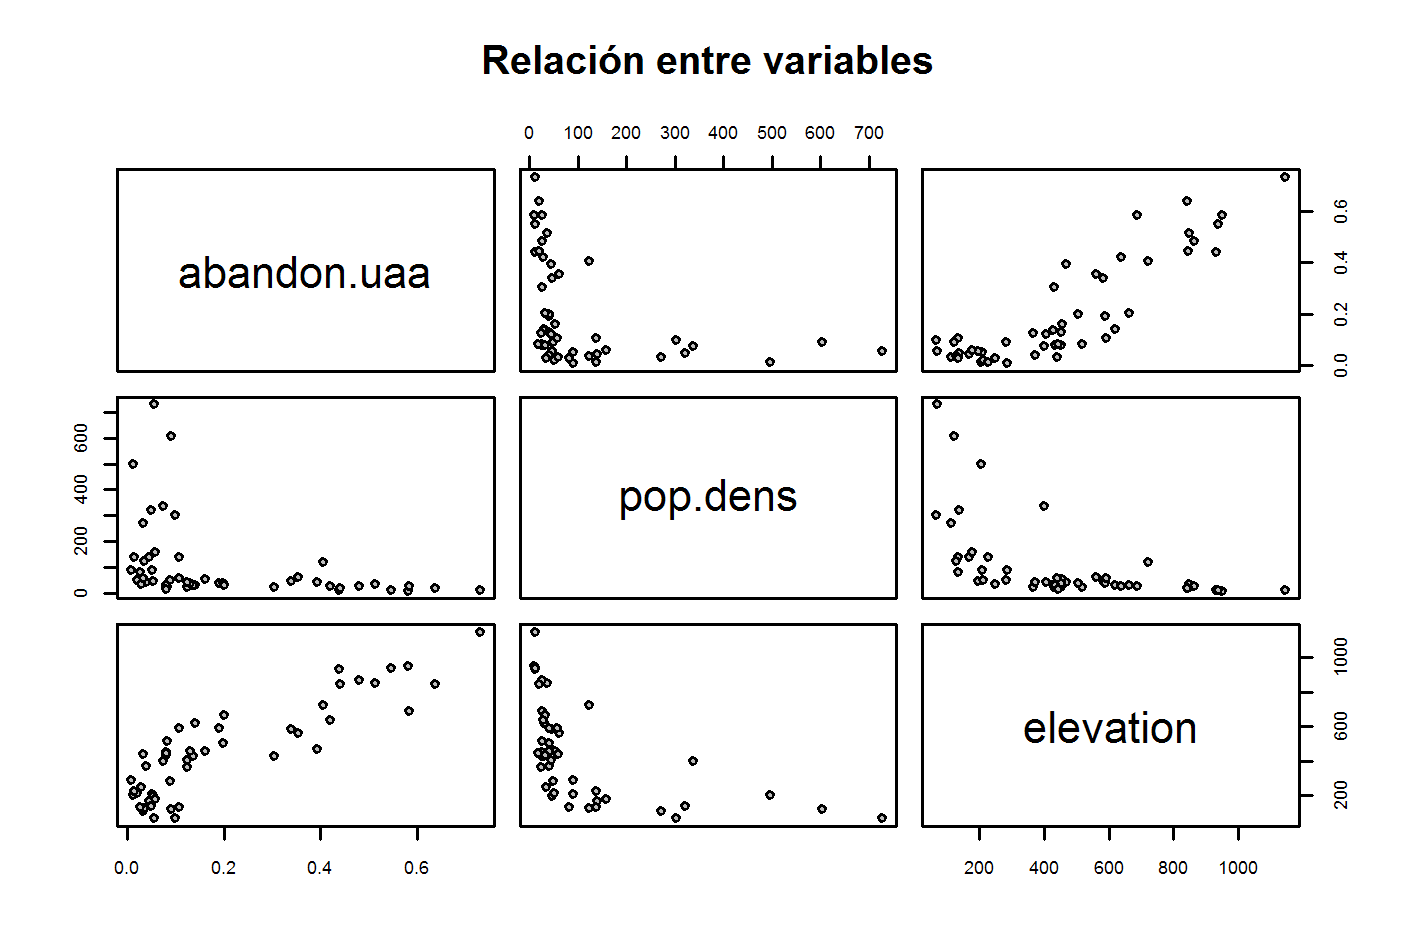
\includegraphics{./R/Graficos/Relacion.png}
	\captionsetup{font={footnotesize,it}}
	\caption{Relación entre variables.}
	\label{fig:relacion}
\end{figure}

\begin{table}[ht]
\centering
\begin{tabular}{rccc}
\toprule[0.4mm]
 & Abandono & Densidad pob. & Elevación\\
\midrule
Abandono & 1 & & \\
Densidad pob. & -0,3620 & 1 & \\
Elevación & 0,8718 & -0,5379 & 1\\
\bottomrule[0.4mm]
\end{tabular}
\captionsetup{font={footnotesize,it}}
\caption{Matriz de correlaciones de las variables.}
\label{tab:matrizcor}
\end{table}

El siguiente paso previo a la generación de agrupamientos sería el de la estandarización de las variables. Tenemos tres variables cuyos datos no se encuentran entre los mismos intervalos donde, por ejemplo, la variable abandono \textit{abandon.uaa} muestra valores entre 0 y 0,73 mientras que la densidad de población (\textit{pop.dens} por ejemplo está entre 9 y 728. Una vez realizada esta estandarización se obtienen los datos del cuadro \ref{tab:estand} donde a cada valor se le resta la media y divide por la desviación típica. Lo que se busca con este estandarizado es el de aproximar los intervalos de los valores de las tres variables y realizar un agrupamiento lo más satisfactorio posible.

\begin{table}[ht]
\centering
\begin{tabular}{rr@{,}lr@{,}lr@{,}lr@{,}lr@{,}lr@{,}l}
\toprule[0,4mm]
& \multicolumn{4}{c}{abandon.uaa} & \multicolumn{4}{c}{pop.dens} & \multicolumn{4}{c}{elevation}\\
& \multicolumn{2}{c}{ant.} & \multicolumn{2}{c}{desp.} & \multicolumn{2}{c}{ant.} & \multicolumn{2}{c}{desp.} & \multicolumn{2}{c}{ant.} & \multicolumn{2}{c}{desp.}\\
\midrule
Mínimo & 0&01 & -0&97 & 9&38 & -0&63 & 67&00 & -1&42\\ 
1$^{er}$ cuartil & 0&05 & -0&74 & 27&47 & -0&52 & 209&80 & -0&90\\
Mediana & 0&11 & -0&47 & 44&50 & -0&40 & 437&00 & -0&06\\
Media & 0&20 & 0&00 & 106&22 & 0&00 & 454&10 & 0&00\\
3$^{er}$ cuartil & 0&35 & 0&75 & 114&55 & 0&05 & 612&00 & 0&58\\
Máximo & 0&73 & 2&66 & 727&83 & 4&07 & 1145&00 & 2&54\\
\bottomrule[0.4mm]
\end{tabular}
\captionsetup{font={footnotesize,it}}
\caption{Valores de las variables antes y después del estandarizado.}
\label{tab:estand}
\end{table}

Pasamos a realizar el agrupamiento jerárquico. Para empezar calculamos la matriz de distancias entre cada observación en tantas dimensiones como variables tenemos, en este caso tres. Para ejercicio aplicaremos el cálculo de una distancia euclídea (cálculo habitual para la distancia entre dos puntos).

Para realizar el agrupamiento se aplica el algoritmo de Ward y obtenemos el dendrograma de la figura \ref{fig:dendro}. En él podemos apreciar los agrupamientos en base a la distancia y el peso de la similitud entre grupos (cuanto mayor es este, menor es la similitud entre grupos). Decidimos realizar los grupos cortando el dendrograma por el peso 5 (línea roja a trazos de la figura \ref{fig:dendro}) resultando así un total de 5 grupos.

\begin{figure}
\centering
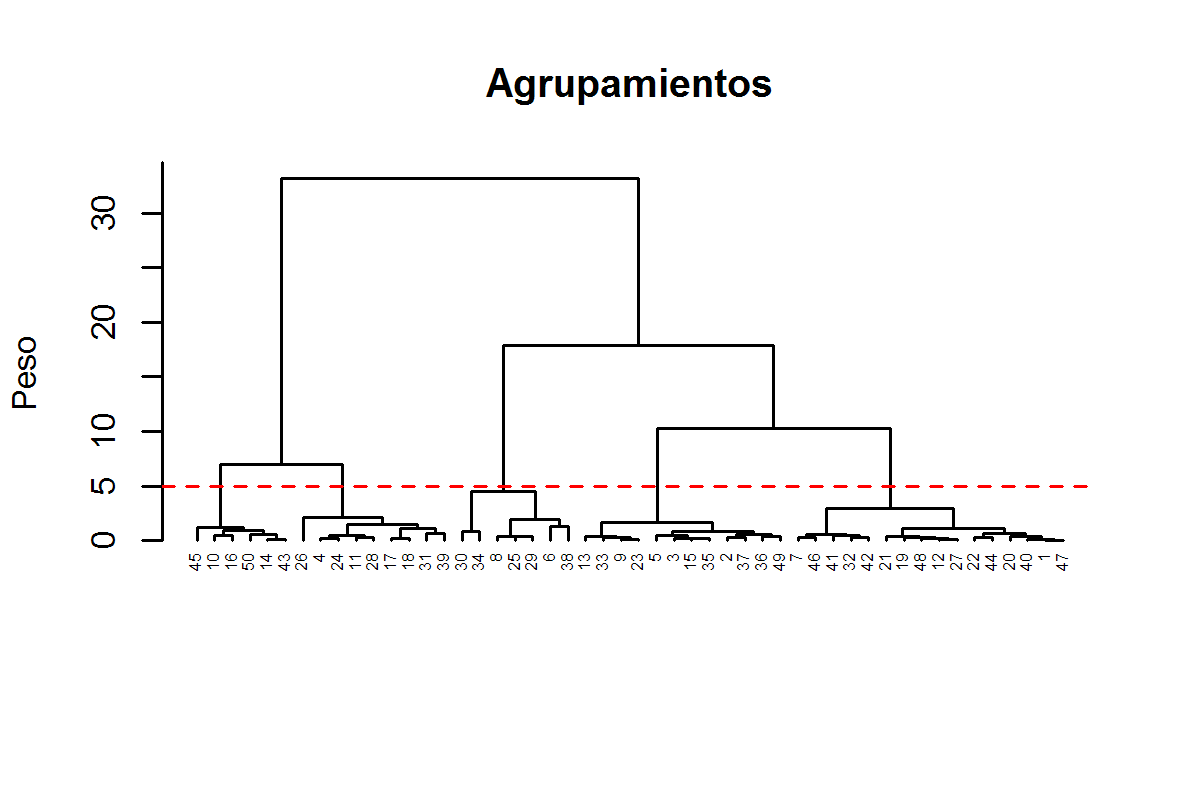
\includegraphics{./R/Graficos/Dendrograma.png}
\captionsetup{font={footnotesize,it}}
\caption{Dendrograma resultante del agrupamiento de observaciones.}
\label{fig:dendro}
\end{figure}

Nos ayudamos de los gráficos de cajas de la figura \ref{fig:box} para analizar los datos de las observaciones por grupos. Extraemos la siguiente información:
\begin{itemize}
\item En la variable abandono los grupos 2 y 4 presentan mucha similaridad y podríamos decir que el grupo 1 se les parece levemente con una media próxima a la de estos otros grupos. Destaca el grupo 3 por ser el más diferente.
\item En cuanto a la variable densidad de población los grupos 1, 3 y 5 se parecen notablemente. Se destaca la gran amplitud de los datos de las observaciones del grupo 4.
\item En la variable elevación hay diferencias en todos los grupos. Los datos están notablemente bien agrupados.
\end{itemize}

\begin{figure}
\centering
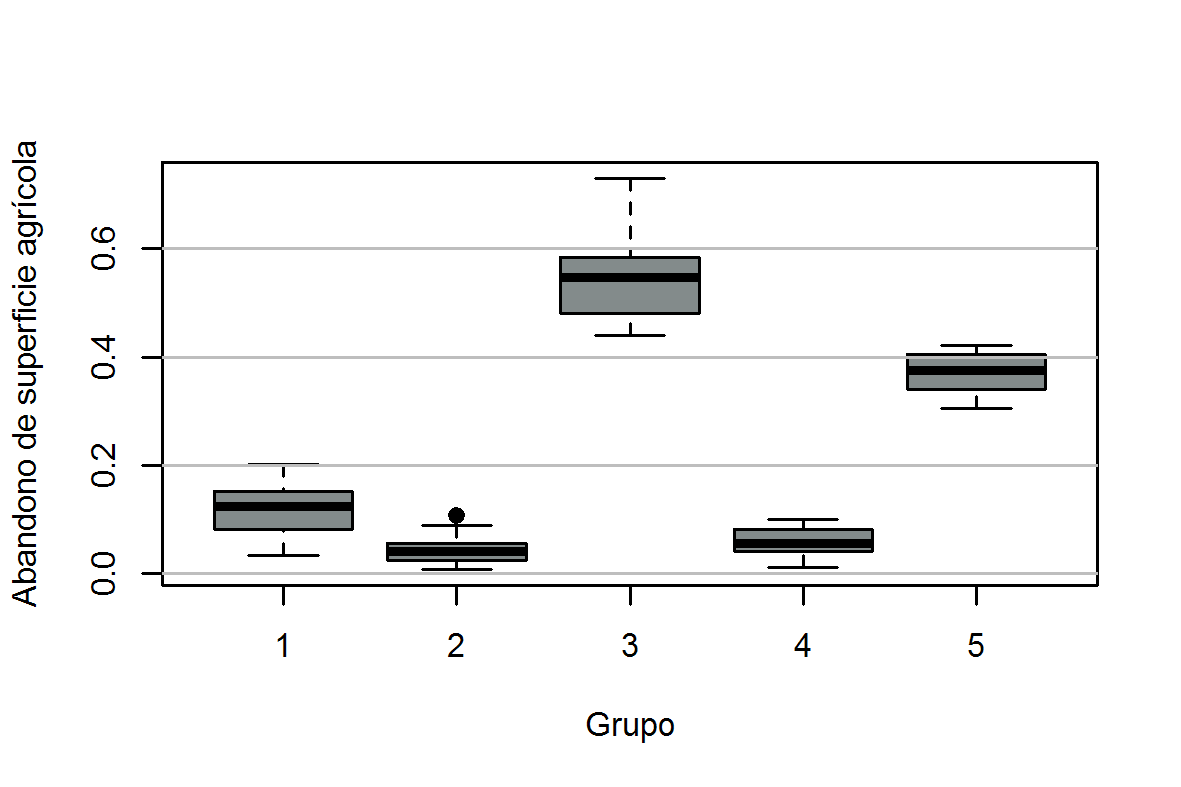
\includegraphics[scale=0.725]{./R/Graficos/BoxAbandono.png}
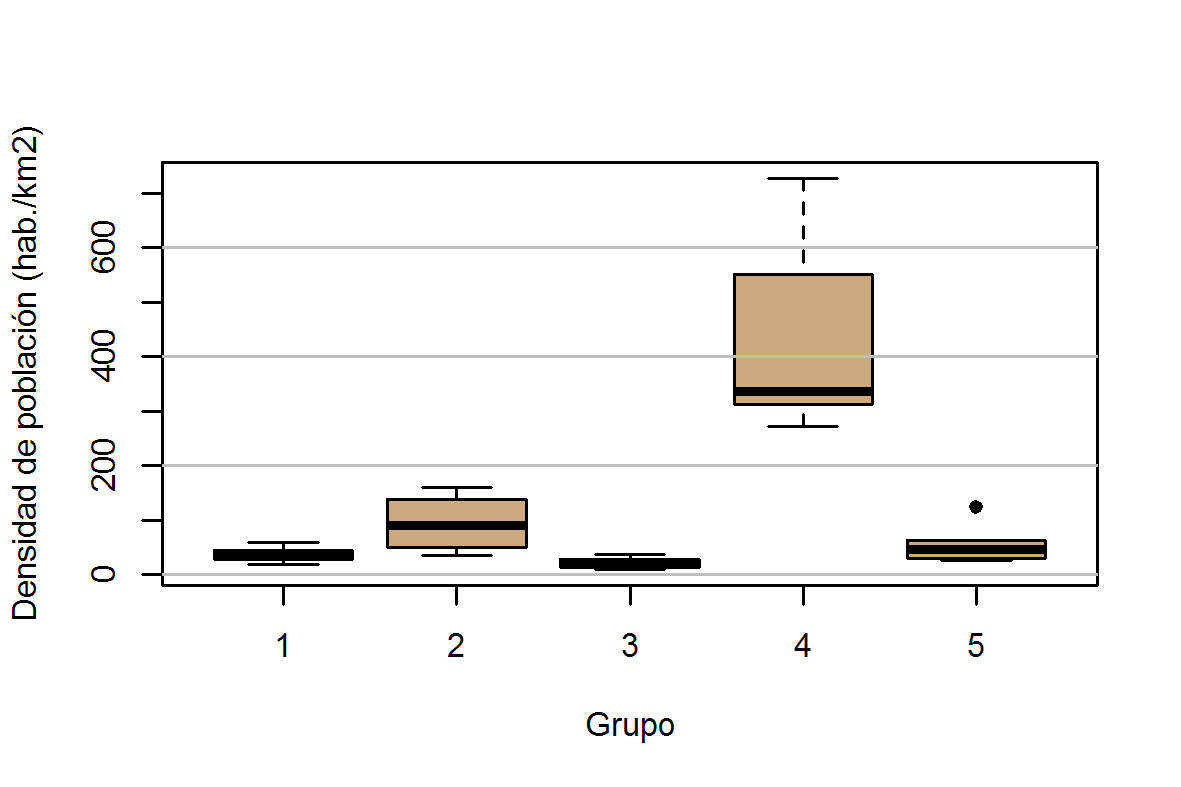
\includegraphics[scale=0.725]{./R/Graficos/BoxDensidad.png}
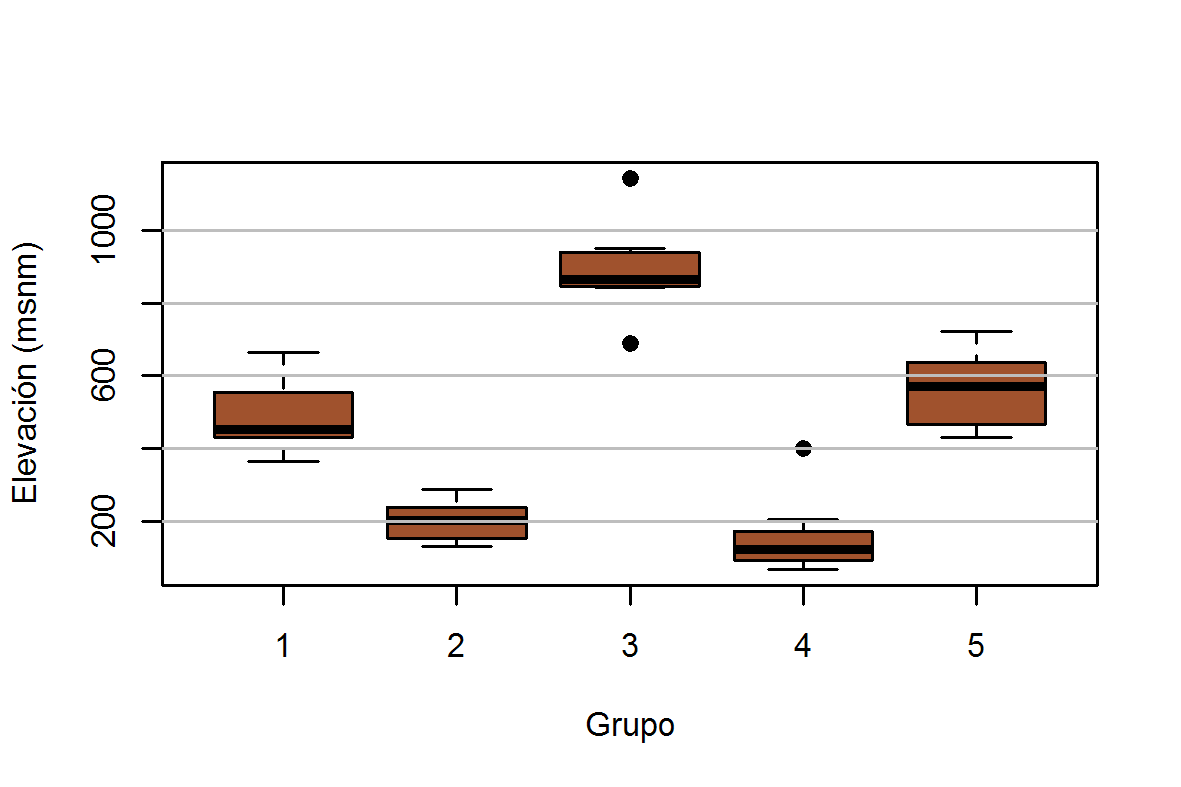
\includegraphics[scale=0.725]{./R/Graficos/BoxElevacion.png}
\captionsetup{font={footnotesize,it}}
\caption{Diagramas de cajas de las observaciones agrupadas.}
\label{fig:box}
\end{figure}

Para realizar un agrupamiento no jerárquico aplicamos el algoritmo \textit{k-means}. Utilizaremos, al aplicar dicho algoritmo, los datos escalados empleados en el agrupamiento jerárquico así como un total de 5 grupos. Adicionalmente, al comparar la coincidencia entre ambos métodos de clasificación resulta el cuadro \ref{tab:comp} En él vemos que las dos agrupaciones son bastante similares (obviando el hecho de que los nombres de los grupos no coinciden) sobre todo en el caso del grupo 4 jerárquico y 3 no jerárquico donde solo se distinguen por una observación agrupada en otro grupo.

\begin{table}[ht]
\centering
\begin{tabular}{cccccc}
\toprule[0.4mm]
Grupos & 1 & 2 & 3 & 4 & 5\\
1 & 0 & 1 0 & 0 & 15\\
2 & 0 & 12 & 0 & 0 & 0\\
3 & 8 & 0 & 0 & 1 & 0\\
4 & 0 & 1 & 6 & 0 & 0\\
5 & 2 & 0 & 0 & 0 & 4\\
\bottomrule[0.4mm]
\end{tabular}
\captionsetup{font={footnotesize,it}}
\caption{Tabla de comparación entre los dos agrupamientos}
\label{tab:comp}
\end{table}

El algoritmo \textit{k-means} crea un número \textit{k} de centroides iniciales, tantos como grupos, originalmente repartidos de forma aleatoria entre las observaciones. Los grupos se generan asignando las observaciones al centroide cuyo valor se aproxime más al valor del dato. El valor del centroide se actualiza al de la media del grupo al que representa y vuelve a realizarse el paso anterior. El proceso es iterativo hasta conseguir convergencia o un número de iteraciones predeterminado.

\end{document}